\documentclass[a4paper,12pt]{article}
\usepackage[T2A]{fontenc}
\usepackage[utf8]{inputenc}
\usepackage[russian]{babel}
\usepackage{graphicx}
\usepackage{float}
\usepackage{subcaption}
\usepackage{amsmath, amssymb}
\usepackage{geometry}
\usepackage{amsmath}
\usepackage{tikz}
\usepackage{hyperref}
\geometry{top=2cm, bottom=2cm, left=3cm, right=1.5cm}

\begin{document}

\thispagestyle{empty}
\begin{center}
    \large
    Министерство науки и высшего образования Российской Федерации\\
    Федеральное государственное автономное образовательное учреждение\\
    высшего образования\\
    «Национальный исследовательский университет ИТМО»\\
    \vspace{5cm}
    \textbf{Отчёт по исследовательской работе № 1}\\
    \textbf{По предмету: Математический анализ и основы вычислений}\\
    \vspace{6cm}
    \begin{flushright}
        Выполнил работу:\\ Тиганов Вадим Игоревич\\
        \vspace{1cm}
        Академическая группа: \\ J3112\\
        \vspace{1cm}
        Вариант: \\18
    \end{flushright}
    \vspace{1cm}
    \vspace{3cm}
    \begin{center}
        Санкт-Петербург, 2025\\
    \end{center}
\end{center}

\newpage


\section{Ход работы}


\subsection{Задание 3}

Требуется:
Найти площадь фигуры, ограниченной кривой \[x^7 + y^7 = ax^3y^3\]

\emph{Графическое изображение фигуры:}
\begin{figure}[H]
    \centering
    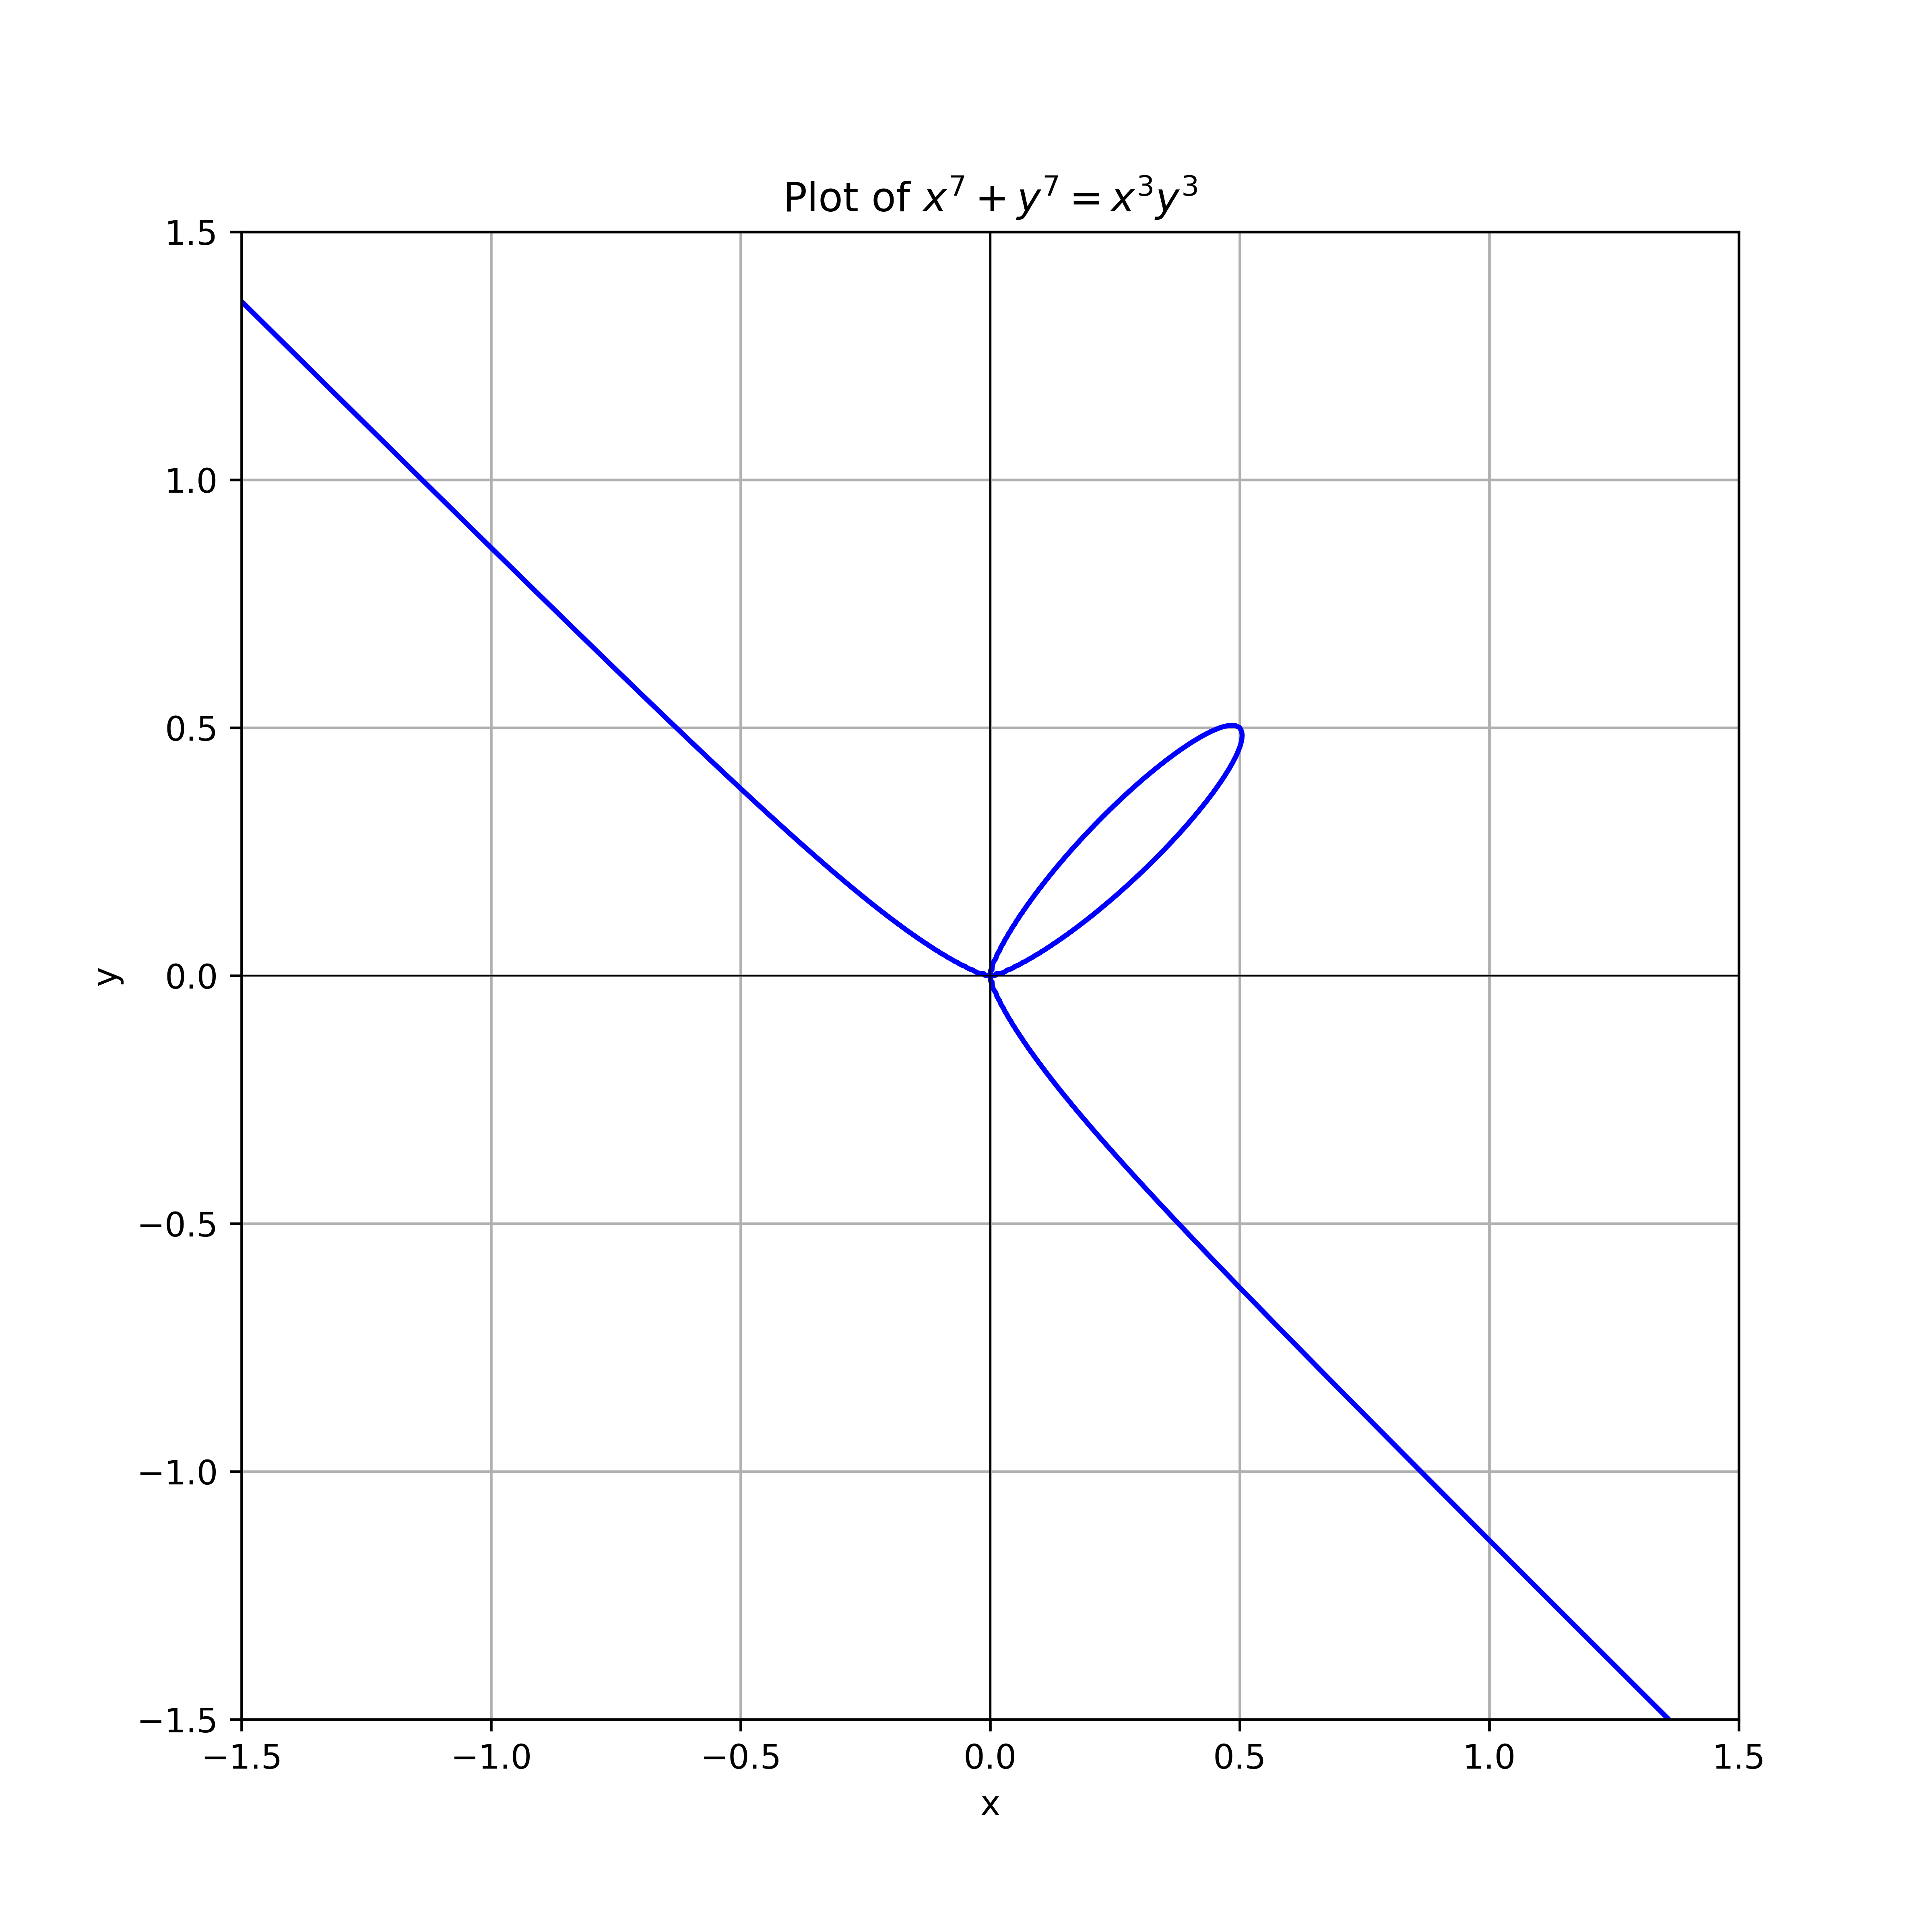
\includegraphics[width=0.9\linewidth]{../img/graph_task4.png}
    \label{fig:integral}
\end{figure}


\emph{Решение задачи:}

\begin{figure}[H]
    \centering
    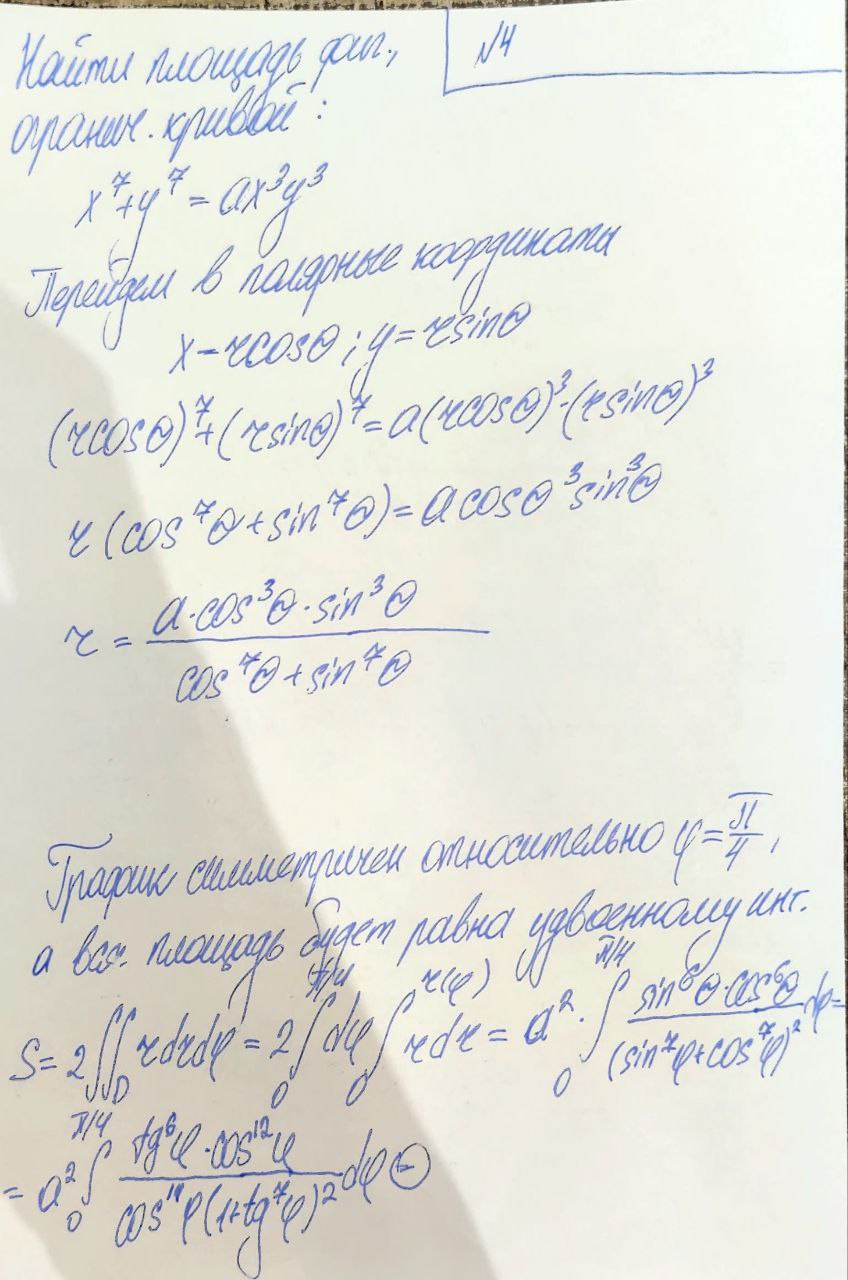
\includegraphics[width=0.8\linewidth]{../img/4_1.jpg}
    \caption{}
    \label{fig:part1}
\end{figure}

\begin{figure}[H]
    \centering
    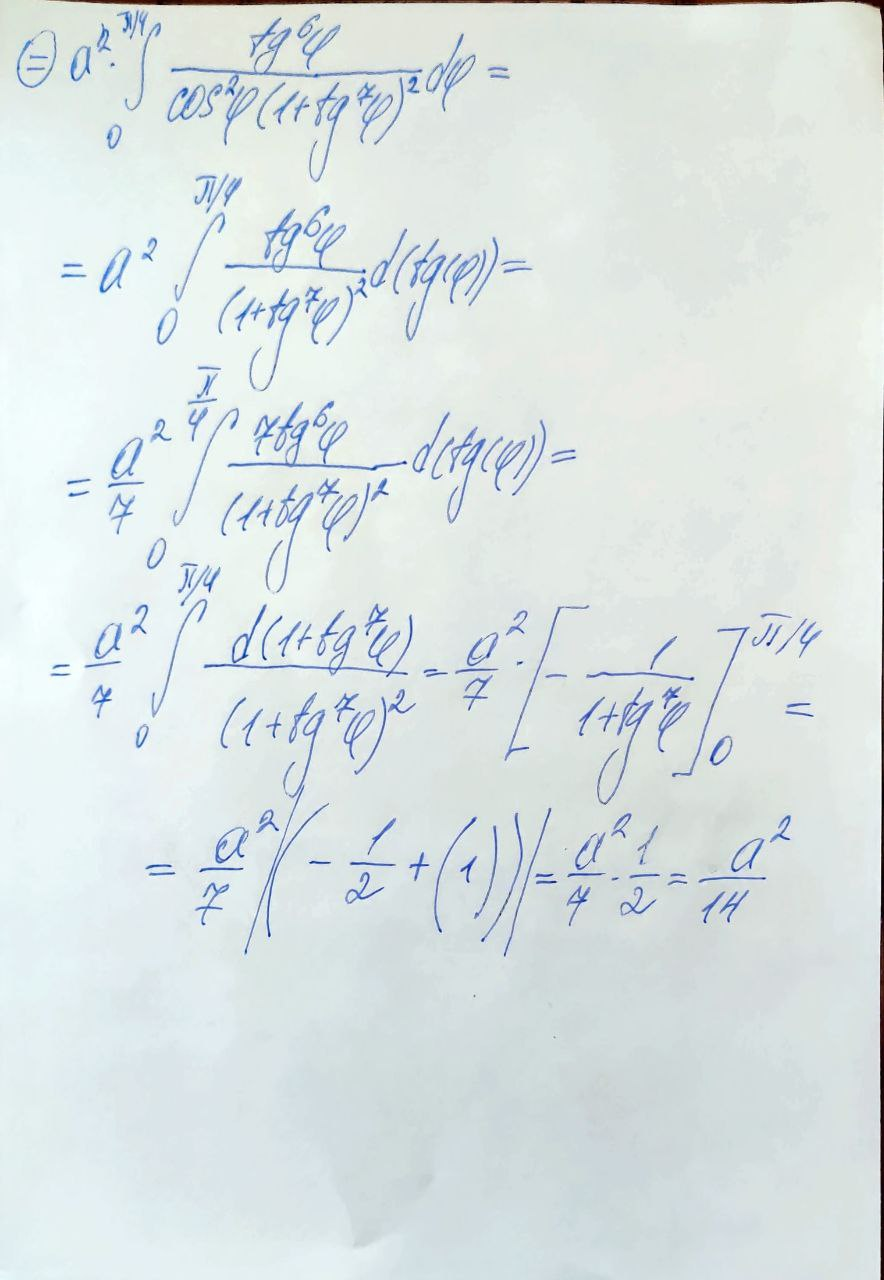
\includegraphics[width=0.75\linewidth]{../img/4_2.jpg}
    \caption{}
    \label{fig:part1}
\end{figure}

\emph{Найденная площадь составила} \( \frac{3a^2}{14} \) \emph{в зависимости от параметра a}.\\
Данная фигура относится к классу алгебраических кривых, а при определенных
значениях параметра может образовывать подобные петли.\\
Для решения задачи и поиска интеграла пришлось использовать нетривиальные
замены и внесение под знак дифференциала, на всех просторах интернета
мне удалось найти только \href{https://primat.org/publ/reshennye_zadachi/vychislenie_ploskoj_figury/43-1-0-775}{единственное решение} подобной задачи --- поиск
площади фигуры, ограниченной кривой \[x^3 + y^3 = axy\]
Делал по аналогии, и все те же замены сошлись, а без перехода к полярным
координатам интеграл не считался. На данный момент была самой сложной задачей, а интеграл проверить я не могу, никакой источник не может посчитать адекватно..


\end{document}